% Chapter 3: Kiến trúc hệ thống
\section{Kiến trúc hệ thống}

\subsection{Tổng quan kiến trúc}
Hệ thống được thiết kế theo kiến trúc module hóa, gồm các thành phần chính:

\begin{figure}[H]
\centering
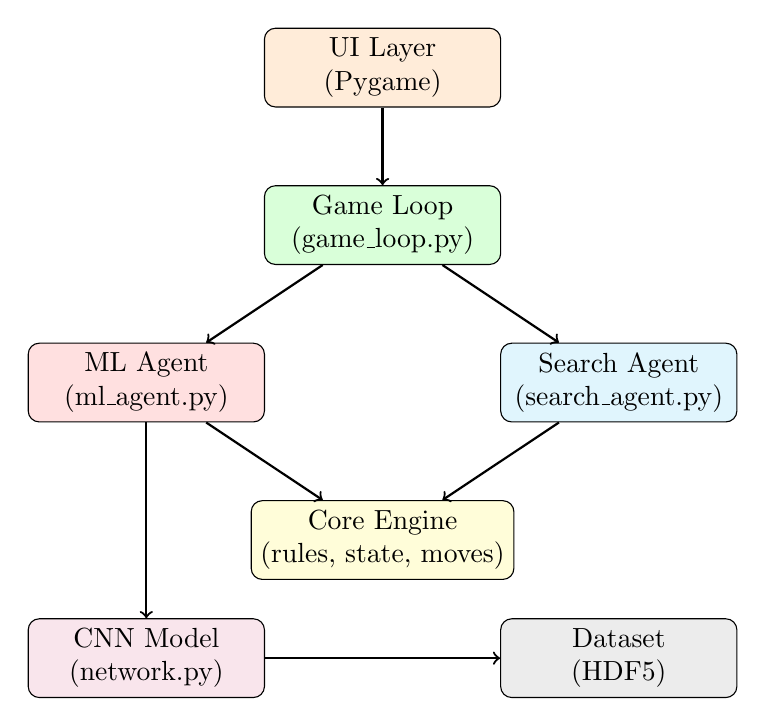
\begin{tikzpicture}[
    box/.style={rectangle, draw, rounded corners, minimum width=3cm, minimum height=1cm, align=center, fill=blue!8},
    arrow/.style={->, thick}
]
\node[box, fill=orange!15] (ui) at (0,0) {UI Layer\\(Pygame)};
\node[box, fill=green!15] (game) at (0,-2) {Game Loop\\(game\_loop.py)};
\node[box, fill=red!12] (ml) at (-3,-4) {ML Agent\\(ml\_agent.py)};
\node[box, fill=cyan!12] (search) at (3,-4) {Search Agent\\(search\_agent.py)};
\node[box, fill=yellow!15] (core) at (0,-6) {Core Engine\\(rules, state, moves)};
\node[box, fill=purple!10] (model) at (-3,-7.5) {CNN Model\\(network.py)};
\node[box, fill=gray!15] (data) at (3,-7.5) {Dataset\\(HDF5)};

\draw[arrow] (ui) -- (game);
\draw[arrow] (game) -- (ml);
\draw[arrow] (game) -- (search);
\draw[arrow] (ml) -- (core);
\draw[arrow] (search) -- (core);
\draw[arrow] (ml) -- (model);
\draw[arrow] (model) -- (data);
\end{tikzpicture}
\caption{Kiến trúc tổng quan hệ thống Xiangqi AI}
\end{figure}

\subsection{Cấu trúc thư mục dự án}
\begin{lstlisting}[language=bash, caption=Cấu trúc thư mục]
xiangqi-ai-project/
|-- agents/           # Cac agent: ML, Search, Random
|   |-- base_agent.py
|   |-- ml_agent.py
|   |-- search_agent.py
|   |-- random_agent.py
|-- core/             # Loi xu ly luat co
|   |-- rules.py      # Enum, luật di chuyển
|   |-- state.py      # GameState (clone, apply, undo)
|   |-- move.py        # Move dataclass
|   |-- move_generator.py  # Legal moves, terminal check
|   |-- encoding.py    # State -> Tensor (15 channels)
|   |-- policy_encoding.py # Move -> Policy index
|-- models/           # ML pipeline
|   |-- network.py     # XiangQiResNet (dual-head CNN)
|   |-- train_fast.py  # Training script
|   |-- preprocess.py  # JSONL -> HDF5
|   |-- dataset.py     # PyTorch Dataset
|-- evaluation/       # Benchmark va danh gia
|-- game/             # Game loop
|-- ui/               # Pygame UI
|-- data/             # Dataset files
\end{lstlisting}

\subsection{Biểu diễn trạng thái bàn cờ (State Encoding)}

\subsubsection{Tensor 15 kênh}
Mỗi trạng thái bàn cờ được mã hóa thành tensor $15 \times 10 \times 9$:

\begin{table}[H]
\centering
\caption{Chi tiết 15 kênh tensor biểu diễn trạng thái}
\begin{tabular}{cll}
\toprule
\textbf{Kênh} & \textbf{Nội dung} & \textbf{Giá trị} \\
\midrule
0 & Tướng (General) phe ta & 1 nếu có quân, 0 nếu không \\
1 & Sĩ (Advisor) phe ta & 1/0 \\
2 & Tượng (Elephant) phe ta & 1/0 \\
3 & Mã (Horse) phe ta & 1/0 \\
4 & Xe (Rook) phe ta & 1/0 \\
5 & Pháo (Cannon) phe ta & 1/0 \\
6 & Tốt (Soldier) phe ta & 1/0 \\
7--13 & 7 loại quân đối thủ (tương tự) & 1/0 \\
14 & Phe hiện tại (Đỏ=1, Đen=0) & 1 hoặc 0 toàn kênh \\
\bottomrule
\end{tabular}
\end{table}

\subsubsection{Canonical Encoding (Chuẩn hóa góc nhìn)}
Để giảm không gian trạng thái, mọi vị trí đều được chuẩn hóa về góc nhìn phe Đỏ. Khi phe Đen đi, bàn cờ được lật 180° (flip hàng). Điều này giúp:
\begin{itemize}
    \item Model chỉ cần học từ một góc nhìn thay vì hai
    \item Giảm 50\% lượng pattern cần nhận diện
    \item Tăng hiệu quả sử dụng dữ liệu
\end{itemize}

\subsection{Policy Encoding (Mã hóa nước đi)}
Mỗi nước đi được mã hóa thành chỉ số trong không gian 8100 chiều:
\begin{equation}
    \text{index} = \text{src\_row} \times 9 \times 90 + \text{src\_col} \times 90 + \text{dst\_row} \times 9 + \text{dst\_col}
\end{equation}
với src là ô xuất phát $(r_1, c_1)$ và dst là ô đích $(r_2, c_2)$. Tổng: $90 \times 90 = 8100$ chỉ số.

\subsection{Data Pipeline}
\begin{enumerate}
    \item \textbf{Thu thập}: CCPD dataset (427MB JSONL, $\sim$120.000 ván cờ thực tế)
    \item \textbf{Xử lý}: Parse FEN + move labels, validate legality
    \item \textbf{Mã hóa}: State → Tensor int8 (15×10×9), Move → Policy index
    \item \textbf{Augmentation}: Horizontal flip (lật gương) × 2 data
    \item \textbf{Lưu trữ}: HDF5 format (chunked, compressed)
    \item \textbf{Kết quả}: 10.208 train + 2.576 val samples (v2), $\sim$1M+ samples (v3)
\end{enumerate}
